%%%%%%%%%%%%%%%%%%%%%%%%%%%%%%%%%%%%%%%%%%%%%%%%%%%%%%%%%%%%%%%%%%%%%%%%%%%%%
%% 02_product_bild03.tex
%% Functional Block Diagram -- CPU Top-Level (TikZ)
%%
%% Shows the five functional blocks of the CPU (dashed) connected by
%% labelled arrows.  Block internals are detailed in subsequent figures.
%%
%% v0.1  2026-06-09  Claude-AI  Initial version
%%%%%%%%%%%%%%%%%%%%%%%%%%%%%%%%%%%%%%%%%%%%%%%%%%%%%%%%%%%%%%%%%%%%%%%%%%%%%

Figure~\ref{fig:asCpuTopBlocks} shows the top-level functional partitioning
of the CPU core.
Each dashed block is detailed in a dedicated diagram in the following sections.

\begin{figure}[H]
\centering
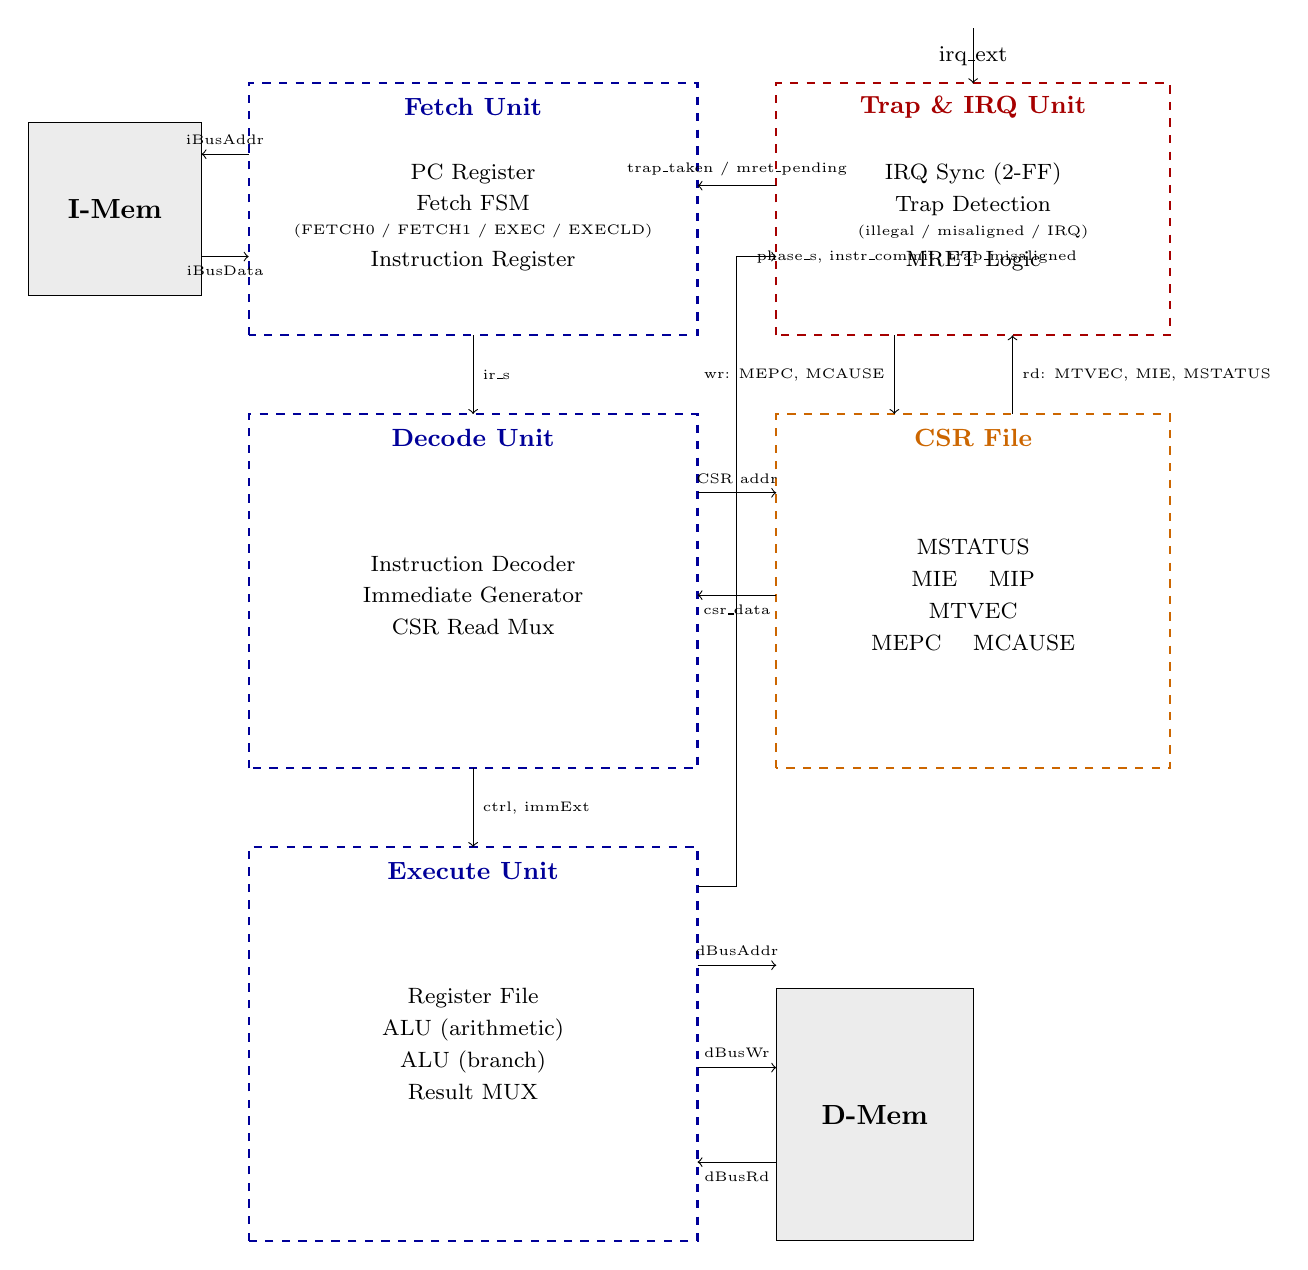
\begin{tikzpicture}[x=1cm, y=1cm]

  % ================================================================
  % External memories (solid boxes)
  % ================================================================

  \filldraw[fill=gray!15, draw=black]
    (0.0, 13.0) rectangle (2.2, 15.2);
  \node[align=center] at (1.1, 14.1)
    {\textbf{I-Mem}};

  \filldraw[fill=gray!15, draw=black]
    (9.5, 1.0) rectangle (12.0, 4.2);
  \node[align=center] at (10.75, 2.6)
    {\textbf{D-Mem}};

  % ================================================================
  % Fetch Unit  (dashed, blue)
  % ================================================================

  \draw[dashed, thick, blue!60!black]
    (2.8, 12.5) rectangle (8.5, 15.7);
  \node[align=center, font=\small\bfseries, blue!60!black]
    at (5.65, 15.4) {Fetch Unit};
  \node[align=center, font=\footnotesize] at (5.65, 14.0)
    {PC Register\\[2pt]
     Fetch FSM\\[-1pt]
     {\tiny (FETCH0 / FETCH1 / EXEC / EXECLD)}\\[2pt]
     Instruction Register};

  % ================================================================
  % Trap \& IRQ Unit  (dashed, red)
  % ================================================================

  \draw[dashed, thick, red!65!black]
    (9.5, 12.5) rectangle (14.5, 15.7);
  \node[align=center, font=\small\bfseries, red!65!black]
    at (12.0, 15.4) {Trap \& IRQ Unit};
  \node[align=center, font=\footnotesize] at (12.0, 14.0)
    {IRQ Sync (2-FF)\\[2pt]
     Trap Detection\\[-1pt]
     {\tiny (illegal / misaligned / IRQ)}\\[2pt]
     MRET Logic};

  % ================================================================
  % Decode Unit  (dashed, blue)
  % ================================================================

  \draw[dashed, thick, blue!60!black]
    (2.8, 7.0) rectangle (8.5, 11.5);
  \node[align=center, font=\small\bfseries, blue!60!black]
    at (5.65, 11.2) {Decode Unit};
  \node[align=center, font=\footnotesize] at (5.65, 9.2)
    {Instruction Decoder\\[2pt]
     Immediate Generator\\[2pt]
     CSR Read Mux};

  % ================================================================
  % CSR File  (dashed, orange)
  % ================================================================

  \draw[dashed, thick, orange!80!black]
    (9.5, 7.0) rectangle (14.5, 11.5);
  \node[align=center, font=\small\bfseries, orange!80!black]
    at (12.0, 11.2) {CSR File};
  \node[align=center, font=\footnotesize] at (12.0, 9.2)
    {MSTATUS\\[2pt]
     MIE \quad MIP\\[2pt]
     MTVEC\\[2pt]
     MEPC \quad MCAUSE};

  % ================================================================
  % Execute Unit  (dashed, blue)
  % ================================================================

  \draw[dashed, thick, blue!60!black]
    (2.8, 1.0) rectangle (8.5, 6.0);
  \node[align=center, font=\small\bfseries, blue!60!black]
    at (5.65, 5.7) {Execute Unit};
  \node[align=center, font=\footnotesize] at (5.65, 3.5)
    {Register File\\[2pt]
     ALU (arithmetic)\\[2pt]
     ALU (branch)\\[2pt]
     Result MUX};

  % ================================================================
  % Arrows
  % ================================================================

  % --- I-Mem <-> Fetch Unit ---
  \draw[->] (2.8, 14.8) -- (2.2, 14.8)
    node[midway, above, font=\tiny] {iBusAddr};
  \draw[->] (2.2, 13.5) -- (2.8, 13.5)
    node[midway, below, font=\tiny] {iBusData};

  % --- Fetch Unit -> Decode Unit (ir_s) ---
  \draw[->] (5.65, 12.5) -- (5.65, 11.5)
    node[midway, right, font=\tiny] {ir\_s};

  % --- Decode Unit -> Execute Unit (control signals) ---
  \draw[->] (5.65, 7.0) -- (5.65, 6.0)
    node[midway, right, font=\tiny] {ctrl, immExt};

  % --- Execute Unit <-> D-Mem ---
  \draw[->] (8.5, 4.5) -- (9.5, 4.5)
    node[midway, above, font=\tiny] {dBusAddr};
  \draw[->] (8.5, 3.2) -- (9.5, 3.2)
    node[midway, above, font=\tiny] {dBusWr};
  \draw[->] (9.5, 2.0) -- (8.5, 2.0)
    node[midway, below, font=\tiny] {dBusRd};

  % --- Decode Unit -> CSR File (CSR address from ir_s) ---
  \draw[->] (8.5, 10.5) -- (9.5, 10.5)
    node[midway, above, font=\tiny] {CSR addr};

  % --- CSR File -> Decode Unit (csr\_data\_s) ---
  \draw[->] (9.5, 9.2) -- (8.5, 9.2)
    node[midway, below, font=\tiny] {csr\_data};

  % --- Trap \& IRQ <-> CSR File ---
  \draw[->] (11.0, 12.5) -- (11.0, 11.5)
    node[midway, left, font=\tiny] {wr: MEPC, MCAUSE};
  \draw[->] (12.5, 11.5) -- (12.5, 12.5)
    node[midway, right, font=\tiny] {rd: MTVEC, MIE, MSTATUS};

  % --- Trap \& IRQ -> Fetch Unit (PC redirect) ---
  \draw[->] (9.5, 14.4) -- (8.5, 14.4)
    node[midway, above, font=\tiny] {trap\_taken / mret\_pending};

  % --- Execute Unit -> Trap \& IRQ (phase, commit, misaligned) ---
  % routed along the right edge
  \draw[->] (8.5, 5.5) -- (9.0, 5.5) -- (9.0, 13.5) -- (9.5, 13.5)
    node[near start, right, font=\tiny] {phase\_s, instr\_commit, trap\_misaligned};

  % --- External IRQ input (top of Trap \& IRQ block) ---
  \draw[->] (12.0, 16.4) -- (12.0, 15.7)
    node[above, font=\footnotesize, yshift=0.1cm] {irq\_ext};

\end{tikzpicture}
\caption{CPU Core -- Top-Level Functional Block Diagram}
\label{fig:asCpuTopBlocks}
\end{figure}
